% !TEX encoding = UTF-8 Unicode

\documentclass[twocolumn,10pt,a4j]{ltjsarticle}
\usepackage{kougai}

\title{ゲームに最適化されたベンチマークソフトの開発}
\author{2032087 大司 陽輝  指導教員 須田 宇宙 准教授}
\date{}

\begin{document}

\maketitle

\section{はじめに}
近年,新型コロナウイルスの影響で自宅で過ごす時間が増えたことにより,PCゲームの需要が増加したことでゲーミングPCの需要が増加している。
しかし,ゲーミングPCの購入やパーツ選択時には,ゲームごとに異なる性能要求を満たす必要があり,自分がプレイしたいゲームに適した性能かどうかを判断する必要がある。コンピューターの性能を評価する方法は多数あるが,ゲームを動かすために必要な処理能力を評価する手段は限られており,既存のゲームベンチマークは特定のゲームタイトルの性能評価に特化しており,異なるゲームの性能比較には適していない。
そこで,本研究では,ゲームによって異なる要素を模し汎用性の高いゲームベンチマークソフトウェアの開発を行う。

\section{ゲームについて}
近年のゲームは,昔に比べリアルなグラフィックに近づけるため,草木などに物理法則に則った動きが追加や,ポリゴン数が増え現状のオープンワールドのゲームではプレイヤーに,約1万7千ポリゴン,サブキャラクターに約5千ポリゴン,敵キャラクターに3千~1万2千ポリゴン使用される,オブジェクトにマッピングされるテクスチャの解像度も高くなり,テクスチャは一枚あたり数MBから数十MBになることが多い.図1は,サンプルとして鮮明感がわかるよう宇宙のテクスチャを用意した.左側の球体は高い解像度のテクスチャを使用し,右側は低い解像度のテクスチャを使用している.高い解像度のテクスチャを使用することではっきりとした絵になり,リアルなグラフィックになるが,GPU・VRAMに負荷が掛かりその負荷のかかり方や量はゲームによって異なる.そこで,ゲームが求める各パーツの性能に対して,性能が劣っていると,画像の描画が遅れ(フレームレートが低下し)スムーズにプレイすることができなくなる.%なったり,描画の品質を落とす必要が出てくる.

既存のベンチマークでは,ゲームごとに掛かる負荷が異なることに対して,負荷の再現度が低い.
既存のベンチマークでは,CPUのみに負荷をかけたり,GPUのみに負荷をかけたり,一つのゲームタイトルのみの参考値しか提示されなかったりと,各ゲームへの参考とするには不十分である.
%物理演算やNPCの思考ルーチンの処理を行うためにCPUの性能を重視するゲームや,影や高いテクスチャの解像度でリアルなグラフィックの処理を行うGPU・VRAMの性能を重視するゲームや,その両方を求められるゲームがある.

\begin{figure}[H]
\begin{center}
 \includegraphics[clip,width=80mm,height=25mm]{sample_01.jpg}
\end{center}
 \caption{テクスチャの解像度の違いによる見え方の違い}
 \label{fig:図1}
\end{figure}
\vspace{-2mm}


\section{実装}
本研究では,CPUへの負荷を模倣するためにオブジェクト数とポリゴン数を変化させる方法を採用した。また,GPUとVRAMに負荷をかけるために,テクスチャの解像度とシェーダーを変更することで,ゲーム環境を再現することが可能であると考察した。そこでソフトウェアの実装はUnityを用いりその様子は図2で示す。

\vspace{1mm}
\begin{figure}[H]
\begin{center}
 \includegraphics[clip,width=80mm,height=35mm]{FlexBench.png}
\end{center}
 \caption{開発を行ったソフト}
 \label{fig:図1}
\end{figure}

そこで本研究では,オープンワールで用いられるキャラクターやモンスターの情報をもとに開発したソフトでポリゴン数を再現し,さらにステージのポリゴン数1万ポリゴン,草や木などのオブジェクトを数個~数十個の1オブジェクトあたり500ポリゴン,シェーダーはUnityで広く用いられる汎用的なStandardシェーダーを使用して,様々な性能のハードウェアで検証を行った結果を図2と,表1の対応表にて示す.図2の数値は,ベンチマークソフト実行時のCPUの使用率を示している.GPUの性能が十分であればCPUの性能がフルに使われるが,GPUの性能が足りていない場合は,CPUの性能が十分に使いきれないため,使用率を監視することで,不足している性能を把握することができる,

\vspace{1mm}
\begin{figure}[H]
\begin{center}
 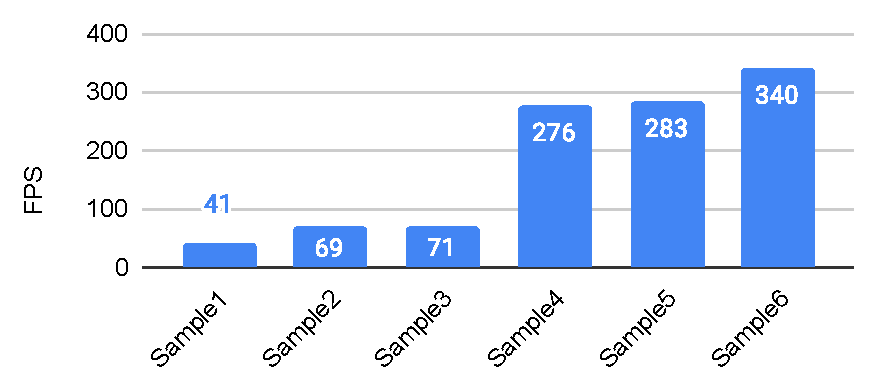
\includegraphics[clip,width=70mm,height=25mm]{グラフ.png}
\end{center}
\vspace{-2mm}
 \caption{各構成でのCPU使用率}
 \label{fig:図1}
\end{figure}

\vspace{5mm}
\begin{table}[H]
\begin{center}
\caption{ハードウェア構成の対応表}
\vspace{2mm}
 \label{fig:教科書}
 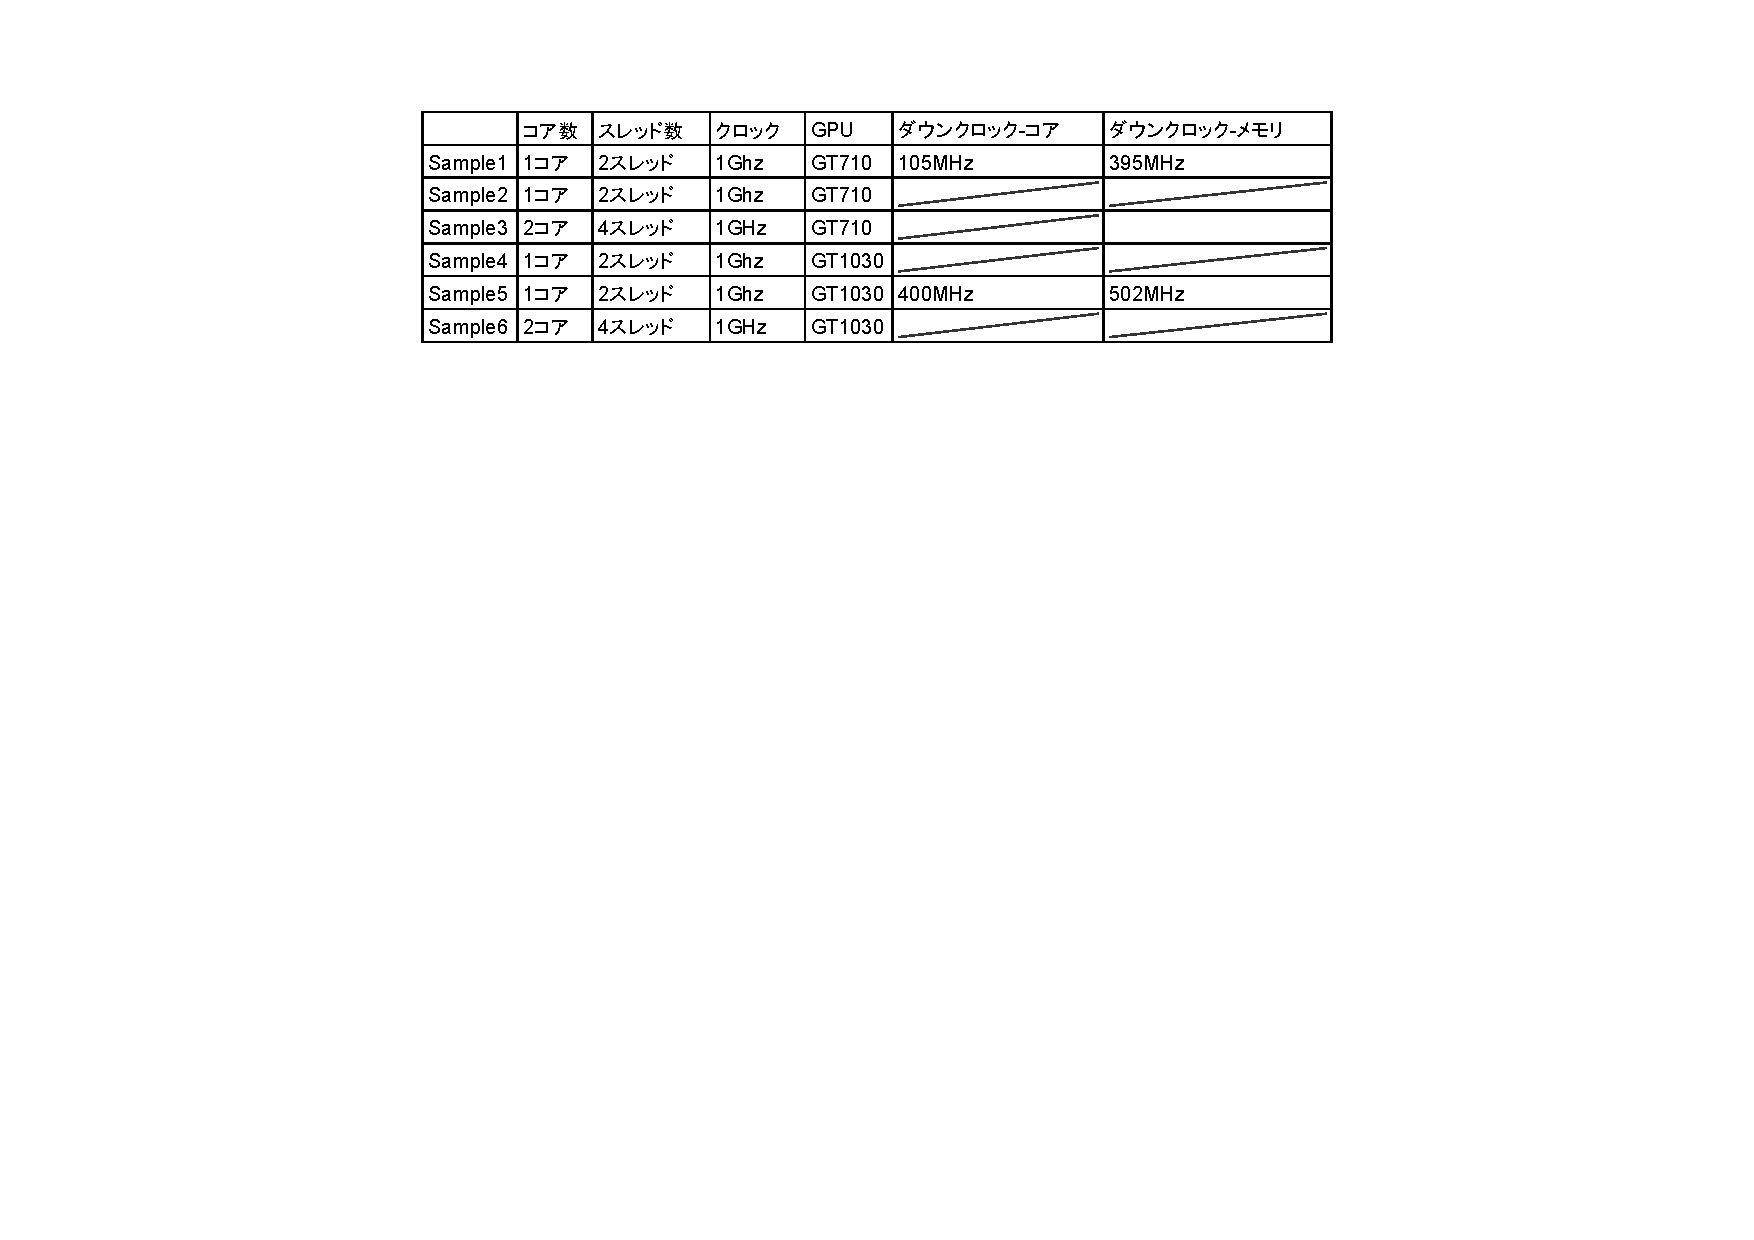
\includegraphics[clip,width=65mm,height=25mm]{対応表.pdf}
\end{center}
\end{table}

\vspace{-5mm}
\section{終わりに}
\vspace{-1mm}
本研究では,ポリゴン数やオブジェクト数を変更できるソフトを開発することで,ゲームの処理を模し,ゲームの負荷を再現することができ不足しているパーツの性能を明確にすることができた.今後は,機能を追加することでさらに忠実にしていきたい.


\end{document}
